\section{Esquemáticos}
\par En esta sección, voy a tratar de encajar algunos de los datos más técnicos del proyecto, sobre todo los referentes a la estructura del sistema y los flujos de información representados.
\par Entre ellos, tengo un prototipo de modelo de datos, esquemas sobre el funcionamiento de Drupal, y una idea de los flujos de información de la visita.

\subsection{Modelo de datos}
\par Hemos dejado bien claro que el propósito de este trabajo no es desarrollar de cero un CMS si no escoger y adaptar uno ya existente a las necesidades que se nos han presentado. Antes de tomar una decisión (que es independiente del autor y tomará tiempo), es conveniente señalar que sí que debería existir una parte de ``diseño original'' que correspondería al modelado de algunas informaciones.


\subsubsection{Catálogo}
\par Respondiendo a los requisitos enunciados por miembros de la empresa, he elaborado un diseño de modelo de datos que podría utilizarse para abstraer los contenidos de un catálogo de objetos expuestos (subconjunto de ítems informativos del total del museo virtual) y no expuestos.
Para ello, me he ayudado de un catálogo editado en papel por el propio Ministerio de Fomento titulado ``Instrumentos históricos del Instituto Geográfico Nacional". Debido a su creación artesanal cada instrumento no sigue la debida canonización que nos piden las bases de datos, y es por eso que he tratado de ordenarlo en un modelo de datos como el que se muestra:

~\paragraph{OBJETO}
\begin{itemize}
\item id/ref: número entero
\item nombre: caracteres(30)
\item firmado: (inventor, lugar\_origen, fecha\_origen) (se eliminaría del original)
\item inventor: relación(n:n)
\item lugar\_origen: relación(n:n)
\item fecha\_origen: fecha
\item dimensiones: caracteres(12)
\item características técnicas: texto
\item materiales: caracteres(20)
\item depósito\_habitual: relación(1:n)
\item observaciones: texto
\item área: relación(1:1)
\item tipo de objeto: relación(1:n)
\item foto: caracteres(50)
\item depósito actual: caracteres(50)
\end{itemize}

~\paragraph{ÁREA}
\begin{itemize}
\item id: numérico
\item nom\_area: caracteres(20)
{Astronomía esférica, Geodesia geométrica, Topografía planisférica y Fotogrametría terrestre.
Topografía altimétrica, Gabinete, Meteorología, Geofísica}
\end{itemize}

~\paragraph{TIPO\_OBJETO}
\begin{itemize}
\item id: numérico
\item nom\_tipo: caracteres(40)
\item id\_area: relación(n:1)
\end{itemize}

~\paragraph{ARTÍCULOS}
\begin{itemize}
\item id: numérico
\item titulo: caracteres(25)
\item contenido: texto
\end{itemize}

~\paragraph{AREA\_ARTÍCULO}
\begin{itemize}
\item id\_area: relación(1:n)
\item id\_articulo: relación(n:1)
\end{itemize}

~\paragraph{INVENTOR}
\begin{itemize}
\item id\_inventor: numérico
\item nom\_inventor: caracteres(25)
\end{itemize}

\par Este modelo será reutilizado (si se aprueba) para crear una interfaz sencilla de entrada de datos para el personal interno.

\subsubsection{Revisión del catálogo}

\par En reuniones posteriores, el cliente indicó que estaban desarrollando un catálogo de instrumentos en papel paralelamente a este proyecto. Este catálogo vendría a dar unas pautas sobre los campos y de algún modo la presentación deseable para, además, el museo virtual.

\par Cabe destacar que el modelo nuevo es obviamente más simplificado, aunque algunas voces dentro de los mandos decisivos del cliente todavía dudan sobre si debería llegarse a un tercer modelo intermedio o no.

\par La idea es tratar de reducir la complejidad, aumentar la integridad y la unicidad de los datos y conseguir, a la vez, una buena coherencia semántica entre los diferentes objetos, artículos explicativos y clasificaciones.

\par En el nuevo modelo, el sugerido para el catálogo en papel, tendríamos los siguientes componentes principales.

~\paragraph{Ficha de objeto}
\par En una página del catálogo, contamos con los siguientes elementos, expuestos, sucintamente en la figura \ref{fig:fichacatalogo}. He añadido una estimación sobre el tipo de datos que podría asimilarse a la estructura propuesta.

\begin{itemize}
 \item Título: (Cadena de caracteres).
 \item Fecha: (Fecha o alguna modificación, dado que algunas son aproximadas).
 \item Constructor: (Cadena de caracteres, posiblemente relacionado con una tabla de autores).
 \item Lugar de origen: (Cadena de caracteres).
 \item Características técnicas: (Campo de texto).
 \item Observaciones: (Campo de texto).
 \item Foto: (Cadena de caracteres dirigida a la ruta del archivo de imagen, o del nodo con las fotos a distintos tamaños).
 \item Dimensiones: (Tripleta de enteros, aunque, en este caso, por su nula utilidad, puede ser almacenado como cadena).
 \item Materiales: (Cadena de caracteres, relacionado con una tabla de materiales).
 \item Lugar actual: (Cadena de caracteres, relacionado con una tabla de lugares, dado que son muy pocos posibles).
 \item Referencia: (Entero, aunque se está dudando si utilizarlo como identificador unívoco).
\end{itemize}

  \begin{figure}[h!]
    \begin{narrow}{-1cm}{-1cm}
      \centering
      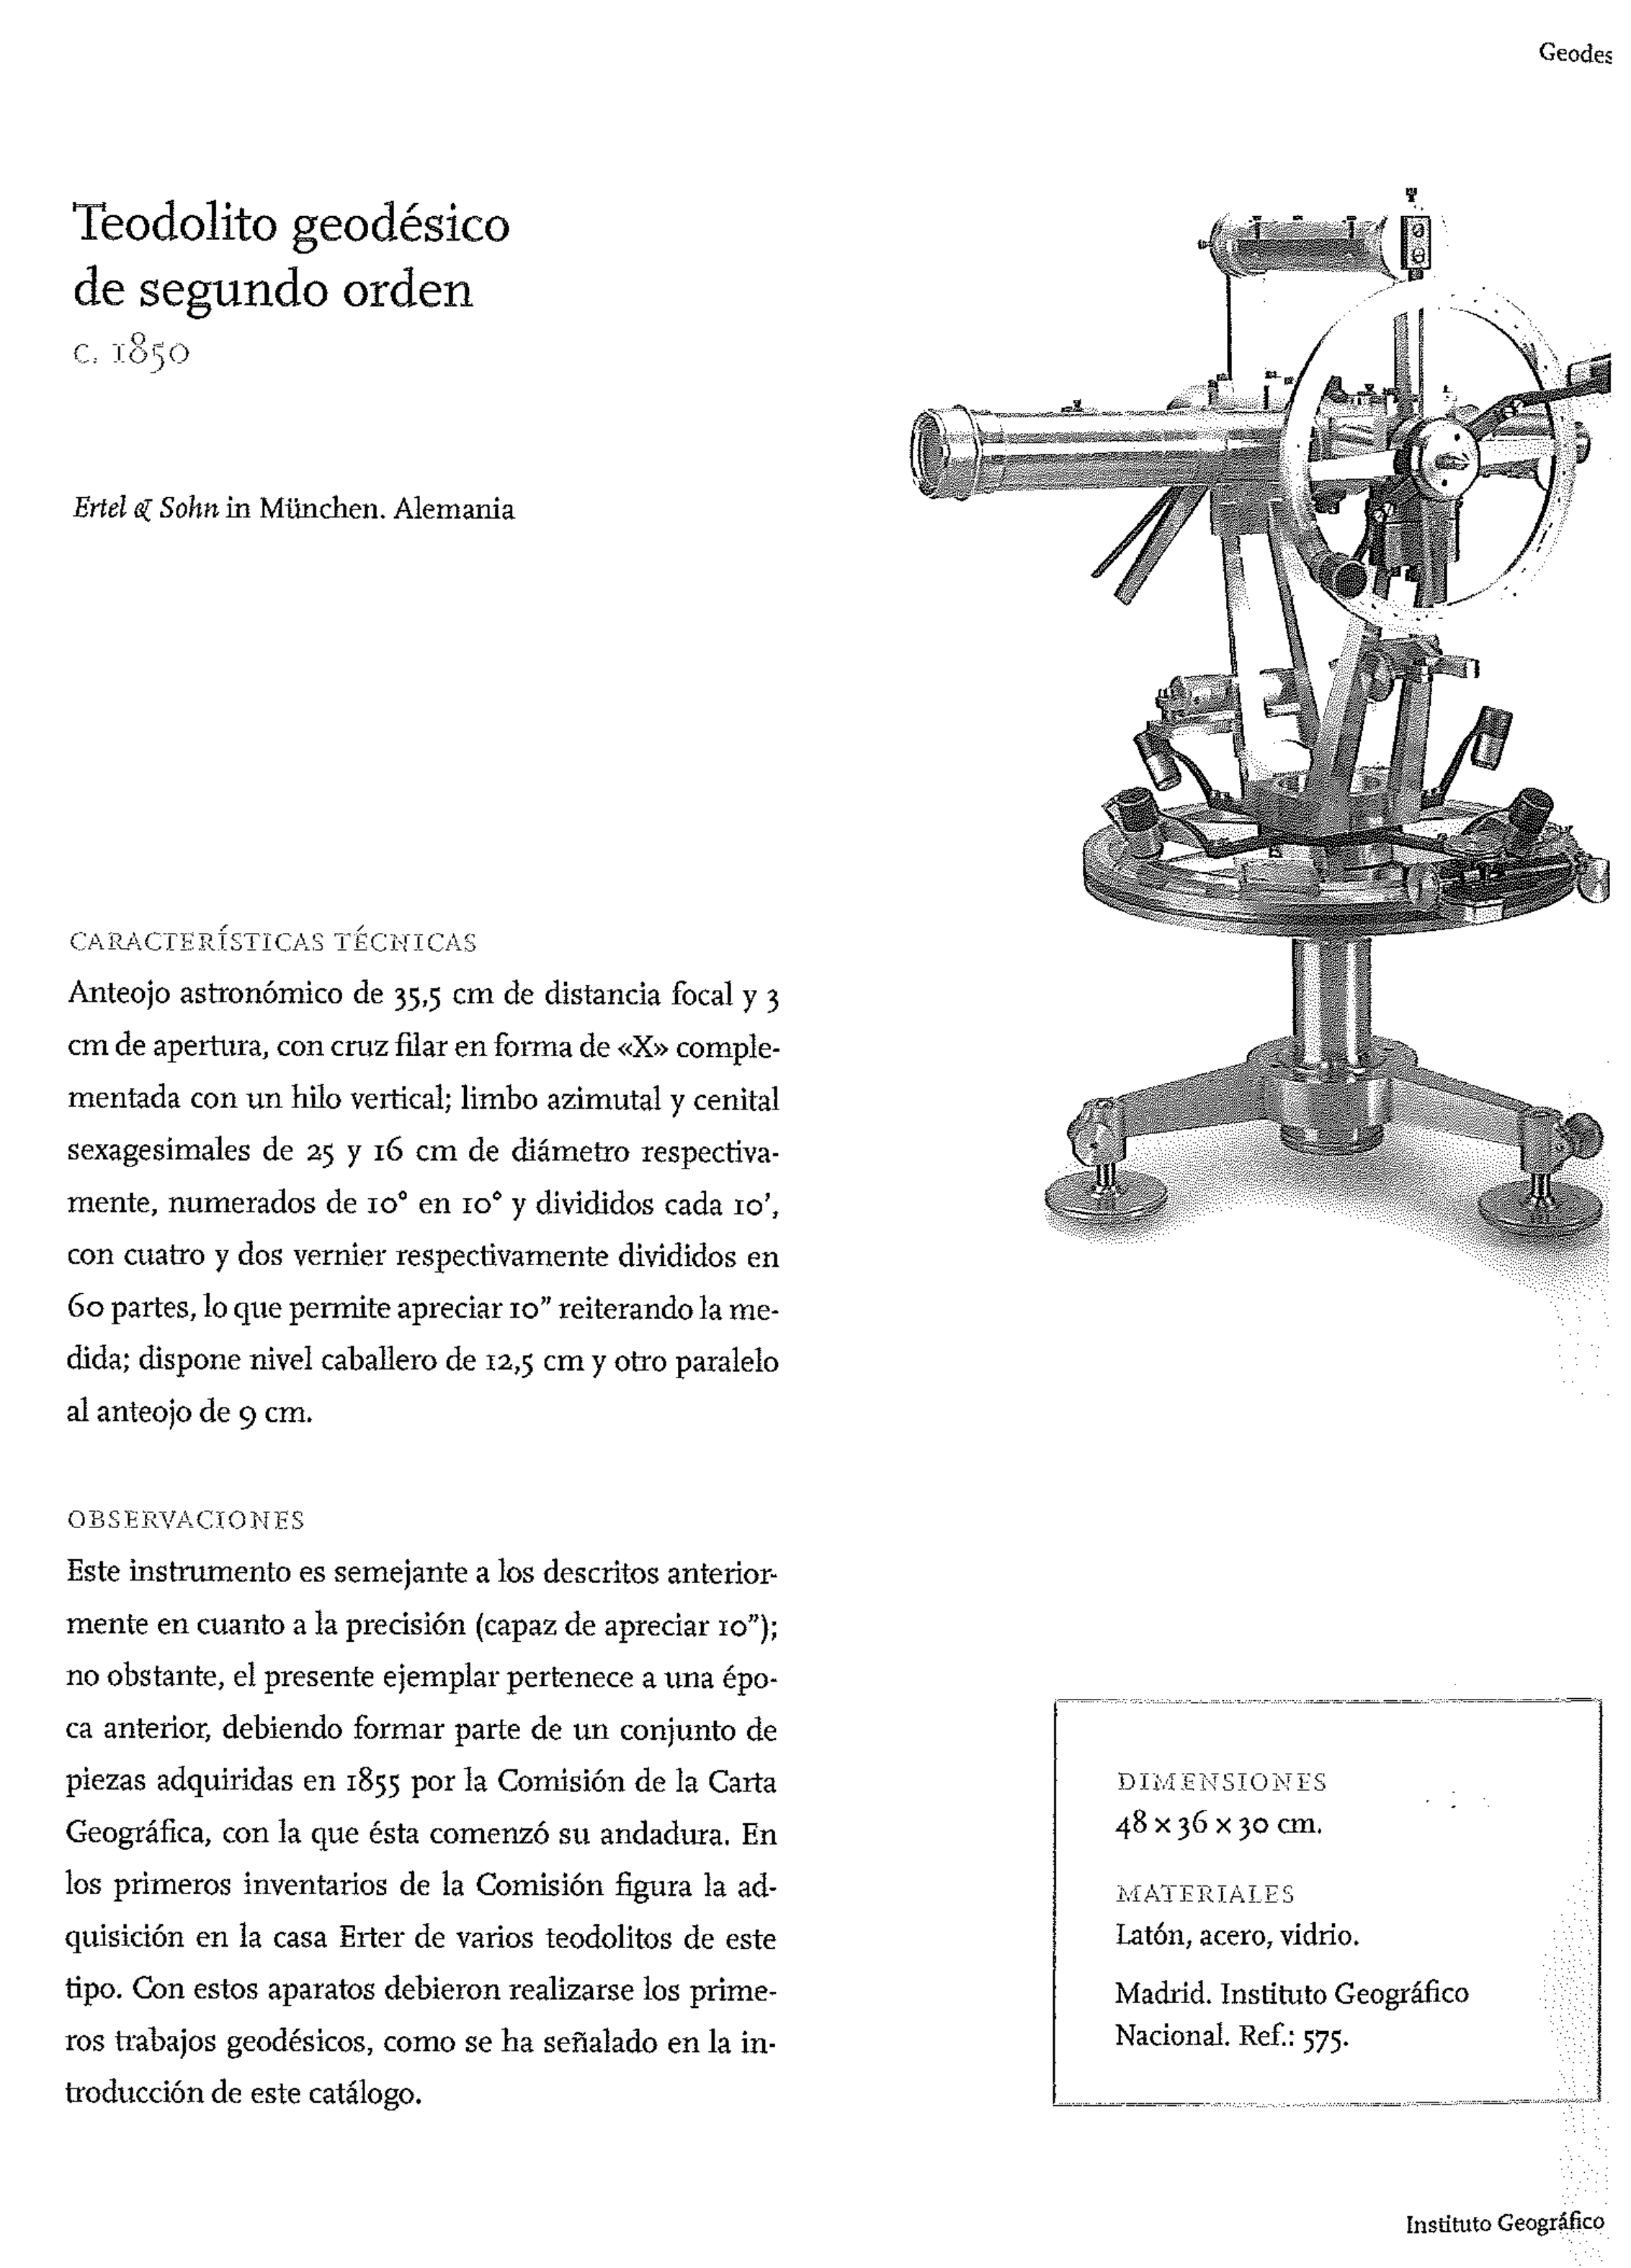
\includegraphics[width=0.8\linewidth]{fichacatalogo}
      \caption{Vista preliminar de una página del catálogo en papel}
      \label{fig:fichacatalogo}
    \end{narrow}
  \end{figure}


\subsection{Esquema general de servicio}
\par En el esquema que se puede ver en la figura \ref{fig:diagen} se describe muy sencillamente la base de funcionamiento del servicio de museo virtual. Especifico que se representa el servicio de museo virtual dado que la parte de generación de contenidos no está presente, dado que ocupará la sección siguiente.

  \begin{figure}[t!]
    \begin{narrow}{-1cm}{-1cm}
      \centering
      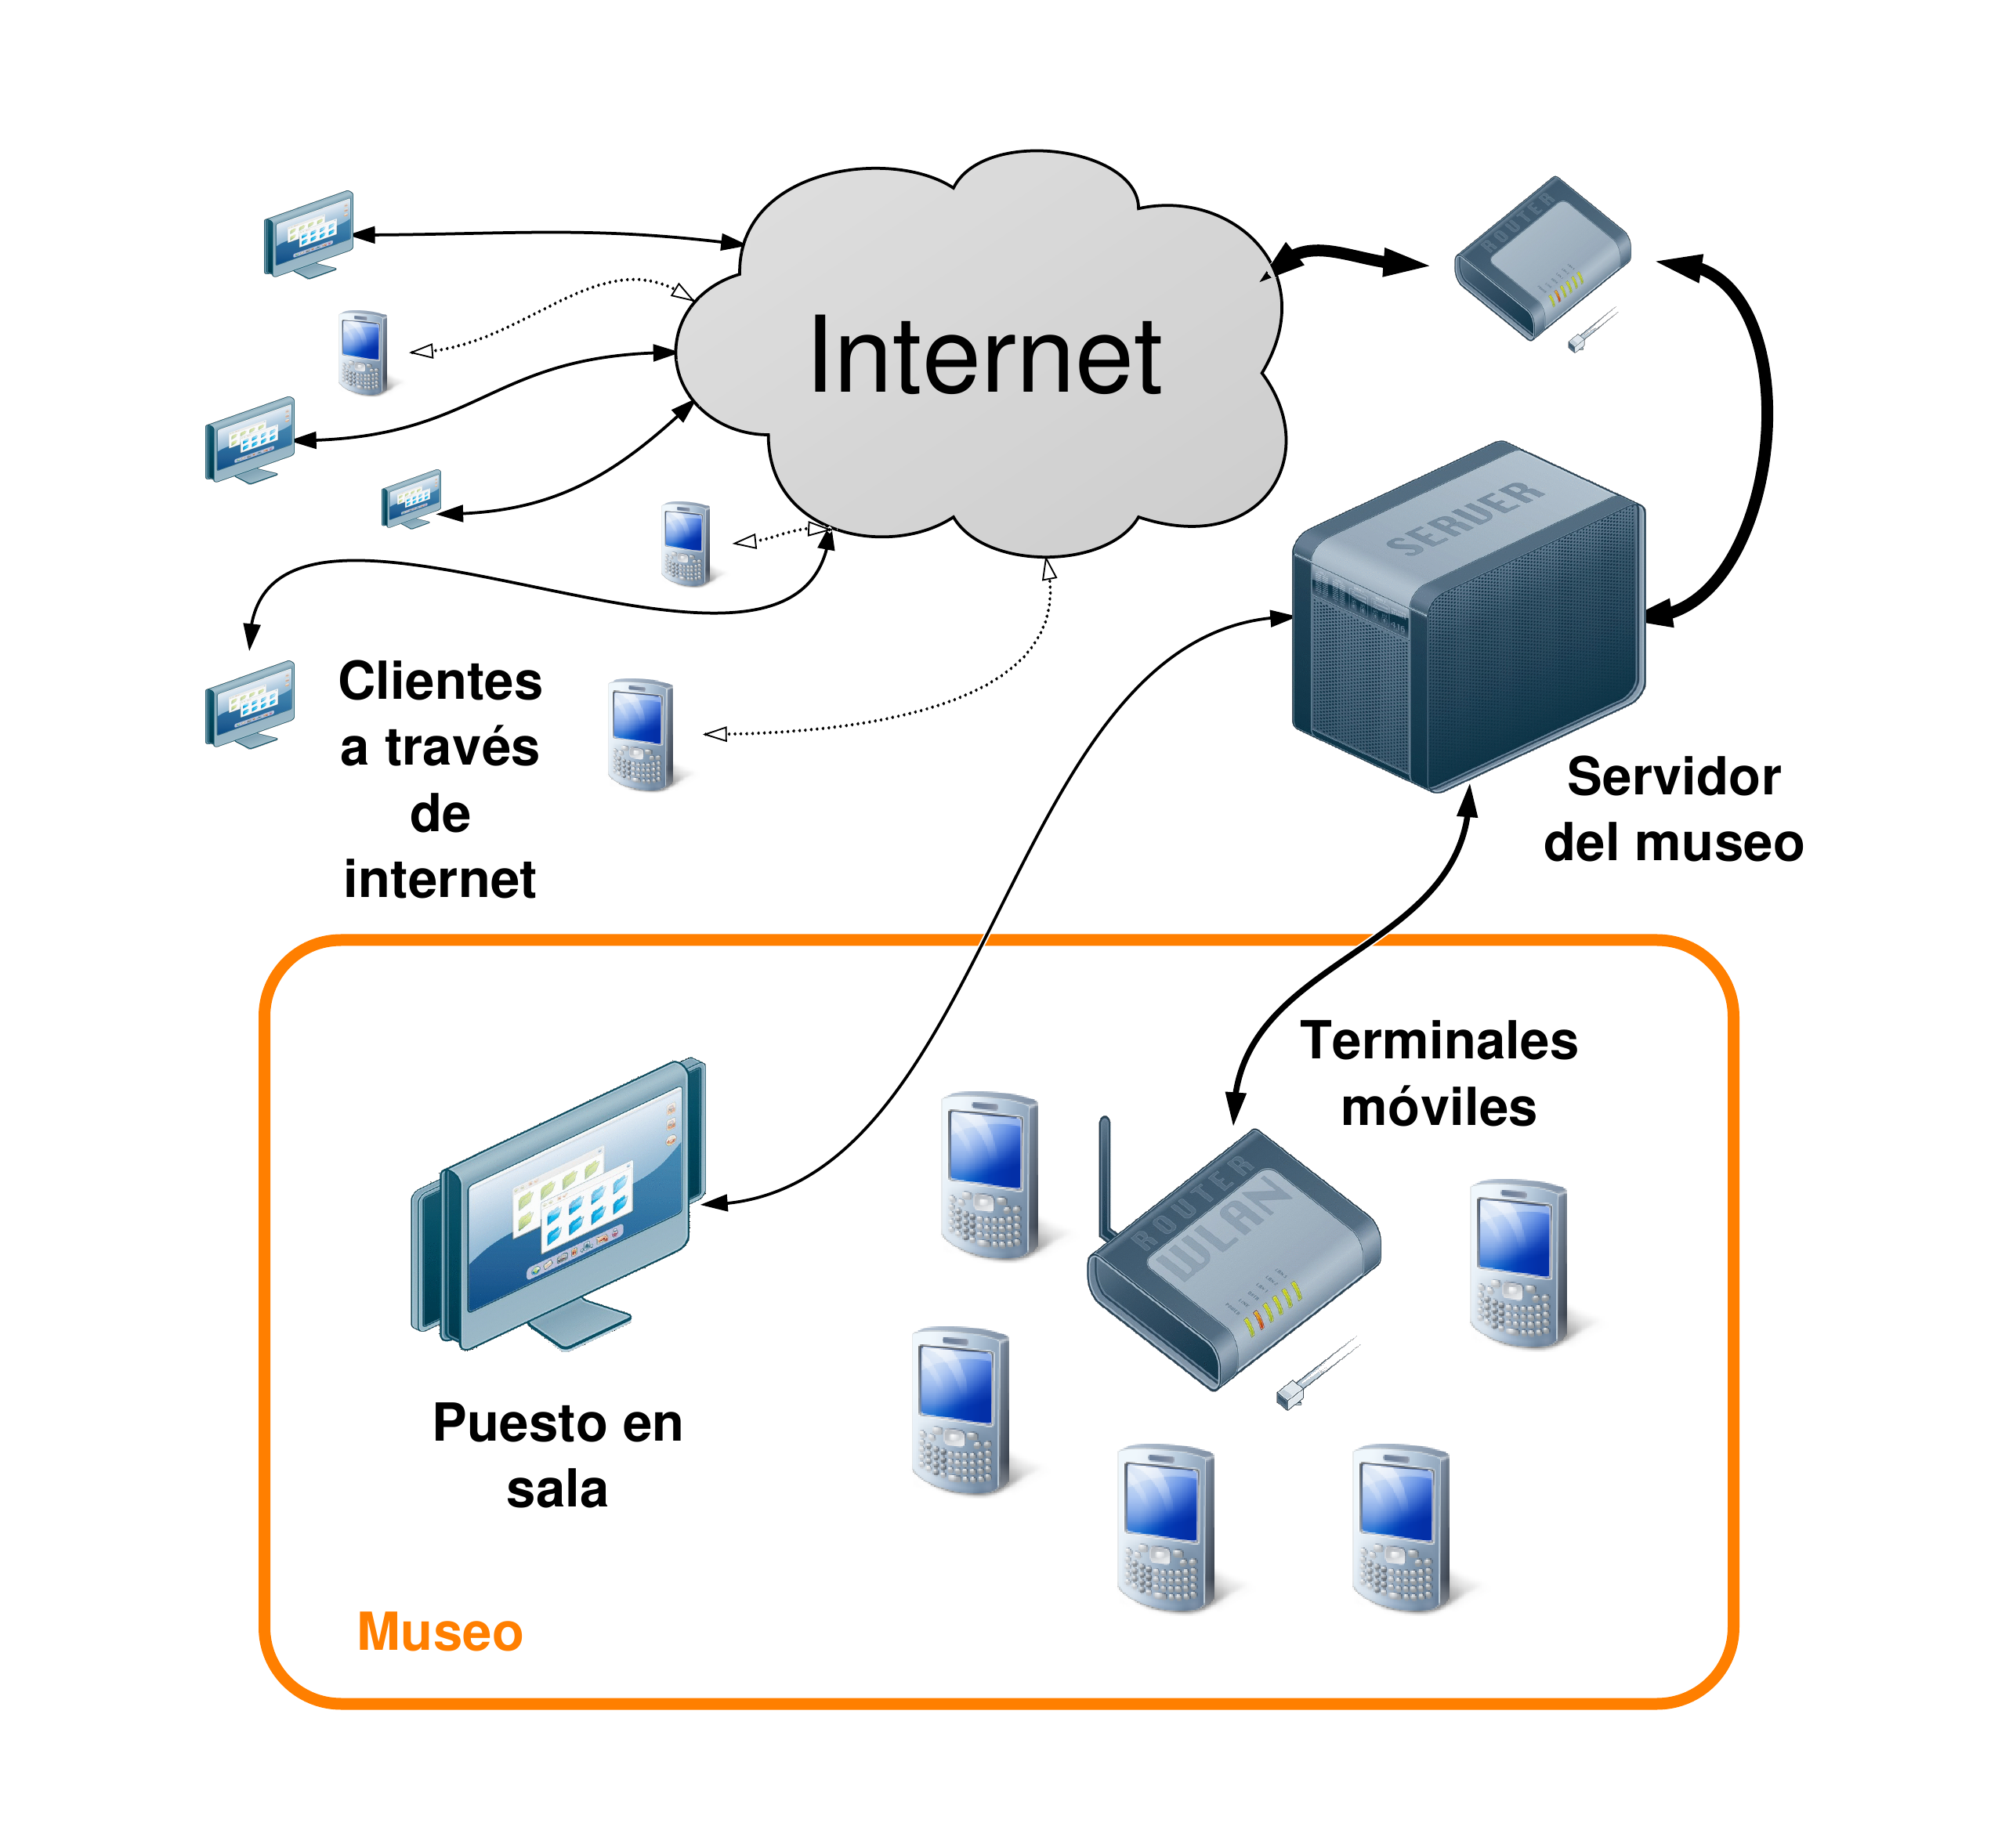
\includegraphics[width=\linewidth]{diagen}
      \caption{Esquema general de servicio}
      \label{fig:diagen}
    \end{narrow}
  \end{figure}

\subsubsection{Servidor del museo}
\par Como ya se ha expresado anteriormente, la idea es tener un único servidor en un principio. Es casi inmediato ver la necesidad de contar con un servidor de pruebas. Además, en un mundo ideal, sería deseable que hubiese una separación entre el servidor de base de datos (con buena parte del contenido textual), el servidor de contenidos multimedia, el servidor de backup y el servidor web propiamente dicho.

\subsubsection{Clientes a través de Internet}
\par La idea es ofrecer a los potenciales o satisfechos visitantes una ampliación a los contenidos vistos en el visita guiada. El porqué de esta decisión es, además de la falta de recursos que requeriría abrir permanentemente al público, que los contenidos de este museo requieren, para ser disfrutados, de una explicación, ya sea textual, audiovisual o hablada, en persona, que es realmente donde más se explota esta posibilidad. Para paliar la falta de tiempo disponible en esta visita, se crea esta alternativa virtual, aunque no se descartan aproximaciones diferentes en un futuro.

\par Para todo esto es necesario que la página esté accesible (tras routers, firewalls, etc.) al gran público a través de Internet y en horario ininterrumpido. Los flujos de comunicación deben ser, en el caso de haber encuestas, cursos o foros, bidireccionales.

\subsubsection{Puesto en sala}
\par Al ser un proyecto ambicioso pero de larga duración, el detalle del número de puestos aún no ha sido delimitado. Aunque pueda parecer una contradicción con las visitas guiadas de público general. Sí que es cierto que pueden proporcionar una herramienta puntual muy útil a la hora de atender a grupos específicos de nivel más avanzado y con más tiempo para detenerse e indagar en la historia de los instrumentos de la colección.
\par Los puestos en sala deberían exclusivamente limitarse a mostrar los contenidos alojados en el servidor, con la salvedad de posibles encuestas, comentarios o sugerencias que saliesen a la luz mientras se usan.

\subsubsection{Terminales móviles}
\par Quizá la parte más novedosa y además, en boga. Estos terminales (tanto privados como alquilados) supondrían una pequeña puerta abierta a visitas más libres y, además, a visitas plurilingües. Sus capacidades de portabilidad, versatilidad e inmediatez a la hora de conseguir contenidos las convierten en un componente idóneo. En el caso del museo, que sería el área de cobertura principal de las mismas, también deberían acceder exclusivamente a contenidos del servidor, evitando cualquier otro camino a tomar dentro de la red. Su capacidad interactiva, por dificultades obvias de comodidad y espacio, podría verse limitada tanto en la versión inalámbrica dentro del museo como en la versión en línea de la misma (que también debe estar disponible al gran público).


\subsection{Esquema general de creación de contenidos}
\par Esta parte quiere detallar el proceso de edición y publicación de contenidos que se seguiría, en en principio en la fase de carga, en caso de que se definiera un esquema colaborativo (actualmente esto está sin determinar). En cualquier caso, la infraestructura estaría preparada para eso; es una característica contemplada en la baremación y la mayoría de sistemas gestores de contenido son válidos para esta cuestión. De hecho, en la sección \ref{cha:usuarios}.

\par Siguiendo el esquema propuesto en la figura \ref{fig:diacreacion}, pasamos a detallar el rol de cada uno de los participantes.

\fig{diacreacion}{Esquema general de creación de contenidos}

\subsubsection{Servidor}
\par Poco que añadir a lo dicho anteriormente salvo reiterar la deseable división de servidores. Una cosa importante sería el decir que la labor de publicación de contenidos recaería directamente sobre el servidor en producción si el esquema propuesto es el colaborativo dado que ese sería un servicio a prestar; o siguiendo el ciclo que describí en la sección \ref{cha:docheckact} si se trata de un esquema estático y unidireccional con una fase de carga de datos única y no cíclica.

\subsubsection{Administrador}
\par Se trataría del mantenedor de la aplicación, siguiendo el mismo ciclo al que hemos hecho referencia en en el párrafo anterior a la hora de implementar cambios que amplíen o modifiquen las funcionalidades requeridas en cada nueva etapa del proyecto. Además, tendrá que prevenir y reaccionar frente a los fallos que puedan ocurrir, tratando de mantener su sistema lo más estable y seguro posible. Incluso, dado la naturaleza inusual del proyecto, deberá dedicarse a optimizar el rendimiento del servidor con las ideas expuestas en el epígrafe \ref{cha:rendimiento}.

\subsubsection{Editor}
\par ''Editor`` se utiliza, en este caso en sustitución de otra designación como podría ser supervisor o coordinador. Normalmente será ocupado por un responsable designado para la tarea que, principalmente y aunque pueda asumir otros roles, como editor, tendrá que revisar los contenidos y dar el visto bueno a cada nueva publicación o modificación. El sistema elegido ya presenta la posibilidad de restringir de esta manera la, llamémosla así, ``versión oficial'' de los contenidos. Quiero incidir en este tema porque es importante que los contenidos presentados por esta plataforma sean fiables, ya que se considera una referencia a nivel nacional (y también de cara a la comunidad internacional) la calidad y fiabilidad de sus textos.

\subsection{Redactor}
\par Como ya hemos venido sugiriendo en los párrafos anteriores, lo que estamos explicando aquí es la parte de ``roles'' que han de asumir los efectivos de los que dispondrá la organización para este proyecto. Esto no supone que deban ser específicamente personas con únicamente ese trabajo. Lo más normal (repito: si se sigue este esquema) es que este rol sea asumido por los profesionales que ya trabajan en el Observatorio, es decir: astrónomos, geofísico, vulcanólogos, cartógrafos, etc.
\par Su rol les permitirá, ya hablando meramente del sistema informático, crear y proponer modificaciones en los contenidos, reservando, como ya hemos dicho, la última palabra y la responsabilidad sobre su publicación definitiva al editor.

